\documentclass[11pt]{article}
\usepackage[T1]{fontenc}
\usepackage{lmodern}
\usepackage[margin=1in]{geometry}
\usepackage{microtype}
\usepackage{amsmath,amssymb}
\usepackage{graphicx}
\usepackage{booktabs,tabularx,array}
\usepackage{enumitem}
\usepackage{xcolor}
\usepackage[most]{tcolorbox}
\usepackage{tikz}
\usetikzlibrary{arrows.meta,positioning,fit,calc}
\usepackage{caption}
\usepackage{needspace}
\usepackage{upquote}
\usepackage[colorlinks=true,linkcolor=blue!50!black,urlcolor=blue!50!black]{hyperref}

\definecolor{plainbg}{HTML}{EEF4FA}
\definecolor{plainframe}{HTML}{2C6FA8}
\definecolor{warnbg}{HTML}{FBF1E6}
\definecolor{warnframe}{HTML}{C07020}

\newtcolorbox{plain}[1][In plain terms]{colback=plainbg,colframe=plainframe,
  fonttitle=\bfseries\small,title={#1},boxrule=0.5pt,arc=2pt,left=6pt,right=6pt,top=4pt,bottom=4pt}
\newtcolorbox{caution}[1][Watch out]{colback=warnbg,colframe=warnframe,
  fonttitle=\bfseries\small,title={#1},boxrule=0.5pt,arc=2pt,left=6pt,right=6pt,top=4pt,bottom=4pt}

\newcommand{\code}[1]{\texttt{\small #1}}
\setlist{itemsep=2pt,topsep=4pt}
\renewcommand{\arraystretch}{1.18}
\captionsetup{font=small,labelfont=bf}

\title{\textbf{The simulation study for the amyloid mixture cure model}\\[4pt]
\large What it checks, how it works, and how to read what it produces}
\author{Guide to the files in \code{simulation/}}
\date{October 2026}

\begin{document}
\maketitle

\begin{plain}[The whole document in one paragraph]
We have a statistical model that reads amyloid PET scans and claims to tell us three things: \emph{whether} a person will ever build up amyloid, \emph{when} they start, and \emph{how fast} they go once they have started. On real patients we can never check whether those answers are right, because nobody knows the true answer for a real person. So we invent patients. We choose the true answers ourselves, use the model's own equations to generate realistic fake scans for 1,101 fake patients, hand those scans to the model as if they were real, and see whether it gives back the answers we put in. We do this many times with fresh fake patients each time, and we keep score. If the model recovers what we planted, that is evidence its answers on real data can be trusted. If it does not, we learn exactly where it goes wrong. The rest of this document explains each step, and the tricks that make it finish in an afternoon on a laptop rather than in a week.
\end{plain}

\tableofcontents
\bigskip

%=====================================================================
\section{Why simulate at all?}

Imagine you buy a kitchen scale and want to know whether it is accurate. Weighing your groceries will not tell you, because you do not know what the groceries really weigh. Instead you put a known one-kilogram weight on it. If it reads 1.00, good. If it reads 1.08, you know it overstates by 8\%. If you repeat with several known weights and it reads a different number each time, you know it is noisy.

A simulation study is the same idea for a statistical model. The real ADNI data are the groceries. The simulated data are the known weights. We know what is in them because we put it there.

There are three specific reasons this model needs the test:

\begin{enumerate}
  \item \textbf{The data are a narrow window onto a long process.} Amyloid builds up over 15 to 20 years, but each person is scanned over a median of about four years. The model has to reconstruct a twenty-year curve from many four-year snippets. It is not obvious that this can be done, and the only way to find out is to try it on data where we know the full curve.
  \item \textbf{The headline result could be an artefact.} The report says APOE4 changes \emph{whether} and \emph{when} people accumulate, but not \emph{how fast}. A model that cannot tell ``started earlier'' apart from ``went faster'' would produce that kind of answer whatever the truth was. We need to check that the model can tell the two apart.
  \item \textbf{Two of the hidden states look identical in the data.} Someone who will never accumulate and someone who has not started yet both have flat scans. The model separates them only through its structure. A simulation tells us whether that separation actually works, and whether the estimated ``never accumulates'' fraction is honest.
\end{enumerate}

\begin{plain}
On real data you only ever see the model's answer. In a simulation you see the model's answer \emph{and} the right answer, side by side. That comparison is the whole point.
\end{plain}

%=====================================================================
\section{A short recap of the model}

You need only the outline of the model to follow the simulation. Every person is, at any age, in one of three hidden states:

\begin{center}
\begin{tabularx}{\textwidth}{@{}l l X@{}}
\toprule
State & Name & What it means \\
\midrule
C & cured & Will never accumulate. Their amyloid sits at a constant personal level for life. \\
L & latent & Will accumulate, but has not started yet. Sits at the shared floor level. \\
P & progressing & Has started. Amyloid is rising along a shared curve. \\
\bottomrule
\end{tabularx}
\end{center}

Three sets of parameters answer the three questions. Each question has its own covariate effects for APOE4 carriage and sex.

\begin{center}
\begin{tabularx}{\textwidth}{@{}l c l X@{}}
\toprule
Question & Symbol & Reported as & Example reading \\
\midrule
Whether: does this person ever accumulate? & $\varphi$ & odds ratio (OR) & OR 5.3 means carriers have 5.3 times the odds of ever accumulating. \\
When: at what age do they start? & $\gamma$ & time ratio (TR) & TR 0.73 means carriers start at 73\% of the age, counted from age 25. \\
How fast: once started, at what speed? & $\psi$ & rate ratio (RR) & RR 1.09 means carriers move 9\% faster. \\
\bottomrule
\end{tabularx}
\end{center}

In equations, for subject $i$ with covariates $x_i$:
\begin{align*}
\text{whether:}\quad & \Pr(\text{ever accumulates}) = \pi_i, \qquad \operatorname{logit}\pi_i = x_i^\top\varphi\\
\text{when:}\quad & \alpha_i = 25 + e^{x_i^\top\gamma}\,E_i^{\sigma_\alpha}, \qquad E_i \sim \text{Exponential}(1)\\
\text{how fast:}\quad & \delta_i = x_i^\top\psi + \sigma_\delta z_i, \qquad z_i \sim N(0,1),\ \text{speed} = e^{\delta_i}\\
\text{the curve:}\quad & G\big(A_i(a)\big) = G(\mu_b) + e^{\delta_i}\,(a - \alpha_i) \quad\text{after departure, flat at } \mu_b \text{ before}\\
\text{the scans:}\quad & y_{ij} = A_i(a_{ij}) + \omega\big(A_i(a_{ij})\big)\cdot t_4 \text{ noise}
\end{align*}
Here $G$ is the ``clock'', a running total of how many disease-years it takes to climb from one level to another. A non-accumulator's curve is simply $A_i(a) = b_i$ for life.

\begin{plain}
Everybody who accumulates rides the same roller-coaster track. People differ in only two ways: when they get on, and how fast their car goes. Some people never get on at all. The model's job is to work out, from a few years of scans each, who got on, when, and how fast.
\end{plain}

%=====================================================================
\section{What the study tries to recover}

A quantity the study scores is called an \emph{estimand}. For every simulated dataset the study records the model's estimate of each estimand and compares it with the truth. There are two kinds.

\subsection{Population-level quantities}

These describe the whole population. They are the numbers that appear in the report.

\begin{center}
\small
\begin{tabularx}{\textwidth}{@{}l X c@{}}
\toprule
Name in output & What it is, in words & Truth (\code{fitted}) \\
\midrule
\code{OR\_apoe4}, \code{OR\_female} & Odds ratio for ever accumulating & 5.32, 1.49 \\
\code{pi\_bar} & Share of the population who ever accumulate, at the cohort average & 0.748 \\
\code{TR\_apoe4}, \code{TR\_female} & Time ratio for when accumulation starts & 0.730, 0.952 \\
\code{RR\_apoe4}, \code{RR\_female} & Rate ratio for speed once started & 1.092, 0.903 \\
\code{mu\_b} & The floor: launch level for accumulators, average level of non-accumulators, in SUVR & 0.585 \\
\code{sigma\_b} & How spread out non-accumulators' flat levels are & 0.059 \\
\code{sigma\_alpha} & How spread out starting ages are & 0.286 \\
\code{sigma\_delta} & How spread out personal speeds are & 0.460 \\
\code{transit} & Years an accumulator spends climbing from the floor to positivity, at average speed & 10.7 \\
\code{cure\_apoe0}, \code{cure\_apoe1} & Share who never accumulate, among non-carriers and carriers & 0.407, 0.114 \\
\code{cross\_apoe0}, \code{cross\_apoe1} & Mean age at crossing the positivity threshold, among accumulators & about 77 and 65 \\
\code{logr\_0.6} \ldots\ \code{logr\_1.5} & The rate curve: log speed of accumulation at ten amyloid levels & see \code{fig\_sim3} \\
\bottomrule
\end{tabularx}
\end{center}

The two crossing ages are slightly different from the rest. Their truth depends on which simulated people happened to be accumulators, so it is computed from each simulated cohort and varies a little from one replicate to the next. Every other truth is fixed by the scenario.

\subsection{Person-level quantities}

These describe individual simulated people. In the simulation we know each person's hidden state, their true starting age $\alpha_i$, and their true speed $\delta_i$.

\begin{itemize}
  \item \textbf{Membership.} For each person, the model gives a probability that they are an accumulator. We check this against who really was one.
  \item \textbf{Starting age.} For true accumulators, we compare the estimated starting age with the true one. We do this separately for people who had already started by the middle of their follow-up (state P) and those who had not (state L). The second group is much harder, because their scans contain no rise to learn from.
  \item \textbf{Speed.} The same comparison for each accumulator's personal speed.
\end{itemize}

\begin{plain}
The population numbers answer ``is the report's table right?'' The person-level numbers answer ``when the model says a particular patient started at 57, how much should we believe it?''
\end{plain}

%=====================================================================
\section{The four scenarios}

A \emph{scenario} is one choice of the true answers. Every scenario starts from the same place, the answers the model gave on the real ADNI data, and changes exactly one thing. Because only one thing changes, any difference between scenarios in how well the model does has a single cause.

\begin{center}
\small
\begin{tabularx}{\textwidth}{@{}l X X@{}}
\toprule
Scenario & What changes from the real-data answers & The question it answers \\
\midrule
\code{fitted} & Nothing. The truth is the model's own answer on real data. & If the world really is as the model says, does the model recover it? \\
\code{rate\_only} & APOE4 no longer changes \emph{when} people start (TR set to 1). Instead carriers go 50\% \emph{faster} (RR set to 1.5). & Can the model tell ``faster'' apart from ``earlier''? \\
\code{low\_cure} & Almost everyone accumulates: 95\% of people, with no effect of APOE4 or sex on that. & Does the model report a 5\% never-accumulate fraction as 5\%, or inflate it? \\
\code{null} & No covariate does anything. All six ORs, TRs and RRs are 1. & How often does the model claim an effect that does not exist? \\
\bottomrule
\end{tabularx}
\end{center}

\paragraph{Why \code{rate\_only} matters most.} The report's central claim is that APOE4 works through ``whether'' and ``when'' and not through ``how fast''. In \code{rate\_only} the truth is the opposite. If the model still reports a time ratio well below 1 and a rate ratio near 1, it is mixing the two up, and the real-data claim cannot be trusted. If it reports a time ratio near 1 and a rate ratio near 1.5, the separation works.

\paragraph{Why 95\% and not 100\% in \code{low\_cure}.} The model's prior belief about the share who accumulate is centred near 72\%. A truth of 100\% sits so far out in that prior that the test would be checking the prior, not the model. Ninety-five percent is extreme enough to expose inflation while staying a fair test.

\paragraph{Why the truths are set at the real-data answers.} Using the model's own estimates makes the fake world look as much like the real one as possible. A check on this: simulated cohorts under \code{fitted} have 41\% and 11\% never-accumulators by APOE4 status, and mean crossing ages near 77 and 65. The report's real-data numbers are 41\%, 11\%, 77.5 and 65.1.

\paragraph{Where this lives.} \code{sim\_truth()} in \code{sim\_truth.R} builds each scenario's parameter list from the posterior medians of the shipped fit. \code{sim\_estimands()} turns a parameter list into the truth values for the population-level table above.

%=====================================================================
\section{How one replicate works}

One \emph{replicate} is one complete trip through the cycle: make a fake cohort, fit the model to it, and score the result. The study repeats this many times per scenario. Each replicate uses fresh random numbers, so each fake cohort is different.

\begin{figure}[h]
\centering
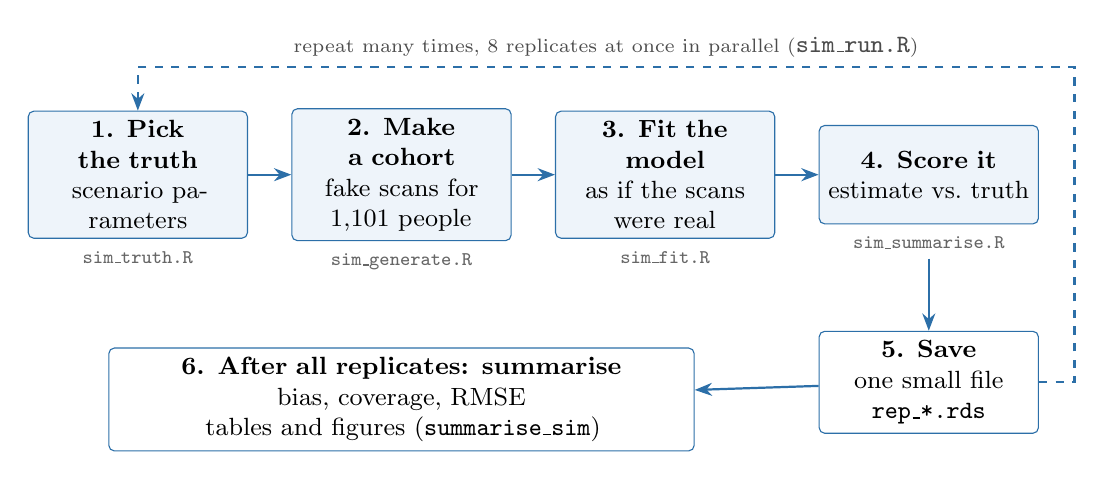
\begin{tikzpicture}[
  box/.style={draw=plainframe, fill=plainbg, rounded corners=2pt, align=center,
              font=\small, minimum height=1.25cm, text width=2.55cm},
  arr/.style={-{Stealth[length=2.2mm]}, thick, plainframe},
  lbl/.style={font=\scriptsize\ttfamily, text=black!60}]
\node[box] (truth) {\textbf{1. Pick the truth}\\scenario parameters};
\node[box, right=0.55cm of truth] (sim) {\textbf{2. Make a cohort}\\fake scans for 1,101 people};
\node[box, right=0.55cm of sim] (fit) {\textbf{3. Fit the model}\\as if the scans were real};
\node[box, right=0.55cm of fit] (score) {\textbf{4. Score it}\\estimate vs.\ truth};
\draw[arr] (truth) -- (sim); \draw[arr] (sim) -- (fit); \draw[arr] (fit) -- (score);
\node[lbl, below=1pt of truth] {sim\_truth.R};
\node[lbl, below=1pt of sim] {sim\_generate.R};
\node[lbl, below=1pt of fit] {sim\_fit.R};
\node[lbl, below=1pt of score] (scorelbl) {sim\_summarise.R};
\node[box, below=1.35cm of score, fill=white] (save) {\textbf{5. Save}\\one small file\\\code{rep\_*.rds}};
\draw[arr] (scorelbl) -- (save);
\node[box, below=1.35cm of sim, text width=7.2cm, fill=white] (sum)
  {\textbf{6. After all replicates: summarise}\\bias, coverage, RMSE\\tables and figures (\code{summarise\_sim})};
\draw[arr] (save) -- (sum);
\draw[arr, dashed] (save.east) -- ++(0.45,0) |- ($(truth.north)+(0,0.55)$)
  node[pos=0.75, above, font=\scriptsize, text=black!70]
  {repeat many times, 8 replicates at once in parallel (\code{sim\_run.R})} -- (truth.north);
\end{tikzpicture}
\caption{The life of one replicate. Steps 1 to 5 run inside one worker process. Many workers run side by side, each on its own replicate.}
\end{figure}

\subsection{Step 2: making a fake cohort}

This is \code{simulate\_cohort()} in \code{sim\_generate.R}.

\paragraph{What stays real.} The fake patients are not made up from scratch. Each one is a real ADNI participant with the same visit ages, the same number of scans, the same APOE4 status and the same sex. Only the amyloid values are replaced with simulated ones. The study therefore asks the right question: does the model work with \emph{this} study's follow-up pattern, scans at these particular ages, rather than with some idealised design. It also makes the compute savings possible, as Section~\ref{sec:fit} explains.

\paragraph{What is drawn for each person.} In this order, using the scenario's true parameters:

\begin{enumerate}
  \item \textbf{Whether.} A weighted coin flip, with probability $\pi_i$ set by their APOE4 and sex, decides whether they will ever accumulate.
  \item \textbf{Their flat level if they never accumulate.} A level $b_i$ near the floor $\mu_b$, never above the positivity threshold.
  \item \textbf{When.} A starting age $\alpha_i$ from the Weibull distribution, between ages 25 and 125.
  \item \textbf{How fast.} A personal speed $e^{\delta_i}$.
  \item \textbf{Their true curve} at each of their real visit ages. Non-accumulators stay at $b_i$. Accumulators stay at the floor until $\alpha_i$, then climb the shared curve at their own speed.
  \item \textbf{The scans.} Each true value plus measurement noise. The noise is larger at higher amyloid levels and occasionally large, matching the Student-$t$ noise the model assumes.
\end{enumerate}

Steps 3 and 4 are drawn for everyone, including non-accumulators, for whom the values are simply never used. This keeps the random-number sequence simple and costs nothing.

\paragraph{Drawing from a restricted range.} Several quantities have limits: a non-accumulator cannot sit above the threshold, a starting age must lie between 25 and 125, and the standardised speed is capped at $\pm 4$. The code respects these exactly by drawing a uniform random number only over the allowed share of the distribution and converting it with the distribution's quantile function. This is the same restriction the model itself assumes, so the fake data obey the model's rules exactly.

\paragraph{The hidden state is recorded.} Each person is labelled C, L or P according to their state at the middle of their follow-up. These labels, along with each person's true $\alpha_i$, $\delta_i$ and curve, are kept for scoring and never shown to the model.

\begin{figure}[h]
\centering
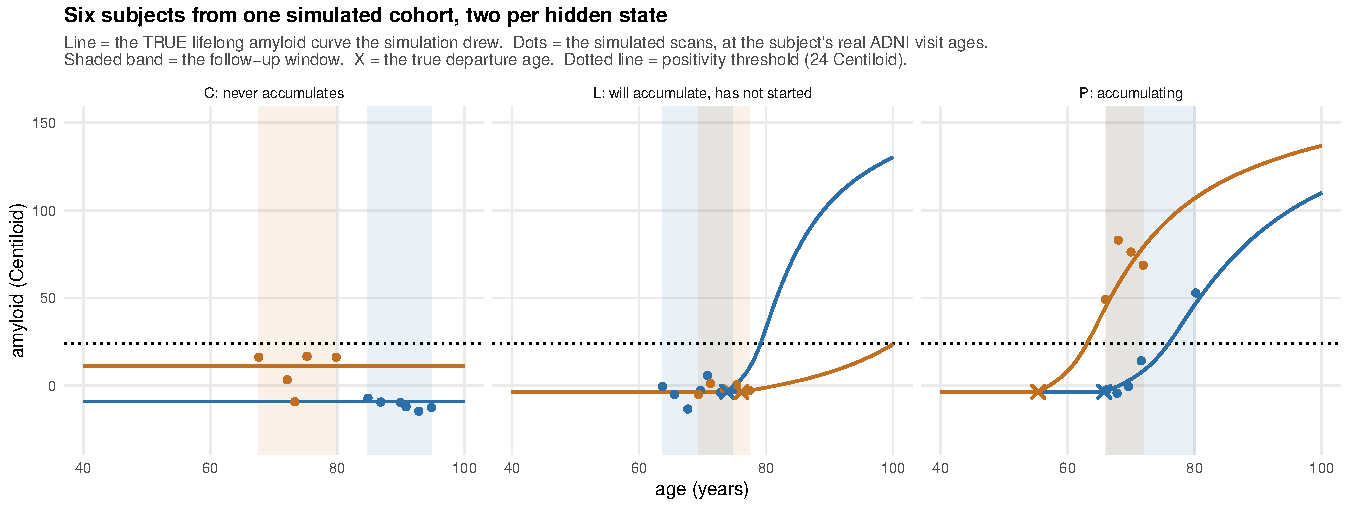
\includegraphics[width=\textwidth]{fig_doc1_cohort.pdf}
\caption{Six people from one simulated cohort under the \code{fitted} scenario, made by the real \code{simulate\_cohort()} code. The model sees only the dots. The simulation also knows the lines, the X marks, and which panel each person belongs in. Notice that the L subjects' scans look just like the C subjects' scans: flat. Only the model's structure can tell them apart.}
\end{figure}

\begin{plain}
For every fake patient we flip a coin to decide if they will ever build up amyloid, roll dice for when they start and how fast they go, draw their true curve, and then blur it with realistic scanner noise at exactly the ages a real ADNI patient was scanned. The model gets only the blurred dots. We keep the answer key.
\end{plain}

\subsection{Step 3: fitting the model}\label{sec:fit}

This is \code{sim\_fit.R}. The model is fitted to the fake scans exactly as it is fitted to real scans: the same model code, the same sampler settings, the same starting rules and the same burn-in. Nothing is tuned for the simulation.

\paragraph{What ``fitting'' means here.} The model is Bayesian. It does not produce one best answer but a large collection of plausible answers, called \emph{posterior draws}, that together describe what the data say and how uncertain they are. These draws come from MCMC, a method that sends a random walker wandering through the space of possible parameter values. The walker spends more time where the values fit the data better. Each fit runs three walkers, called \emph{chains}, from slightly different starting points. If all three end up exploring the same territory, that is a sign the walk has run long enough.

\paragraph{The big time-saver: build once, use many times.} Before NIMBLE can fit the model it translates the model into C++ and compiles it. On the full cohort that takes about 70 seconds. The compiled model depends on the design (who was scanned when, and their covariates) but not on the scan values. Since the design is identical in every replicate, each worker compiles the model once, at the start. For each new replicate it simply swaps the new fake scan values into the already-compiled model and runs it again. This is \code{sim\_compile()} followed by repeated calls to \code{sim\_fit()}.

\begin{plain}
Compiling is like setting up a factory production line. It takes a while, but once the line is built you can feed it batch after batch. A naive simulation would rebuild the factory for every batch. This one builds it once per worker and then just changes the raw materials.
\end{plain}

\paragraph{Where the walkers start.} The chains start from values computed from the fake data, the same rule used on real data. They never start from the truth. Starting at the right answer would hide the case where the walkers have trouble finding it, and would make the model look better than it is. Chains 2 and 3 start from small random nudges of chain 1's start, so that their agreement means something.

\paragraph{A fix for impossible starting points.} The data-based starting rule places each person at the average of their own scans. Occasionally a fake person's average is so high, for example because one scan caught a large noise spike, that the starting curve runs off the top of the model's amyloid range before their last visit. That makes the starting point impossible, and the fit cannot begin. \code{feasible\_inits()} finds those few people and lowers their starting level step by step until every person is possible. This changes only where the walkers begin, not what they are looking for. Real ADNI subjects never trigger it, because none averages that high.

\paragraph{What is kept.} For each chain the sampler records every draw of the population parameters and every twentieth draw of each person's hidden quantities. The first third of each chain is thrown away as warm-up, as in the main analysis.

\subsection{Step 4: scoring the fit}

This is \code{score\_replicate()} in \code{sim\_summarise.R}. For each population-level quantity it records three numbers from the posterior draws:

\begin{itemize}
  \item the \textbf{estimate}: the posterior median, the middle of the plausible values;
  \item the \textbf{95\% credible interval}: the range holding the middle 95\% of plausible values;
  \item the \textbf{truth} for this replicate.
\end{itemize}

For the person-level quantities it uses the package's own \code{subject\_quantities()} routine on 100 draws, and records:

\begin{itemize}
  \item each person's estimated probability of being an accumulator, compared with who really was one;
  \item the error and interval coverage of each accumulator's estimated starting age, split by true state P and L;
  \item the same for each accumulator's speed;
  \item two versions of the correlation between starting age and speed, explained in Section~\ref{sec:pitfall}.
\end{itemize}

It also records R-hat for every parameter. R-hat compares the three chains: close to 1 means they agree; well above 1 means they have not yet settled on the same answer. Recording it lets us later separate ``the model is wrong'' from ``the model was not run long enough''.

\paragraph{Only a small summary is saved.} The full chains for 200 replicates would fill gigabytes and answer nothing further. Each replicate saves only its scores, its R-hat values, a thinned sample of 400 population draws, and its run time, in one small file.

%=====================================================================
\section{Summarising across replicates}

One replicate tells you almost nothing. Any single estimate can land a little high or a little low by chance. What matters is how the estimates behave \emph{across many} replicates. \code{summarise\_sim()} reads every saved replicate for a tier and computes, for each scenario and each quantity, the measures below. They follow the standard reference for simulation studies, Morris, White and Crowther (2019).

\subsection{The performance measures}

Write $\hat\theta_r$ for the estimate in replicate $r$, $\theta_r$ for the truth, and $R$ for the number of replicates.

\begin{center}
\small
\begin{tabularx}{\textwidth}{@{}l l X@{}}
\toprule
Measure & Formula & What it tells you \\
\midrule
Bias & $\frac1R\sum_r(\hat\theta_r - \theta_r)$ & On average, does the model aim too high or too low? Ideally 0. \\
Relative bias & bias $/$ average truth & The same, as a percentage of the true value. \\
Empirical SE & $\operatorname{SD}_r(\hat\theta_r)$ & How much the estimate jumps around from one dataset to the next. \\
RMSE & $\sqrt{\frac1R\sum_r(\hat\theta_r-\theta_r)^2}$ & Typical size of the error, combining bias and jumpiness. \\
Coverage & share of $r$ with truth inside the interval & Do the 95\% intervals contain the truth about 95\% of the time? \\
Mean width & average of (upper $-$ lower) & How precise the intervals are. Narrow is good only if coverage holds. \\
\bottomrule
\end{tabularx}
\end{center}

\begin{plain}[{In plain terms: bias, spread and coverage}]
Think of shooting at a target. \textbf{Bias} is whether your shots are centred on the bullseye or drift off to one side. \textbf{Empirical SE} is how tightly your shots cluster. \textbf{RMSE} is your typical distance from the bullseye, whatever the reason. \textbf{Coverage} is about honesty rather than accuracy. Each time, the model draws a ring around its shot and says ``I am 95\% sure the bullseye is inside this ring''. If it is telling the truth, the bullseye should be inside about 95 rings out of 100. If it is inside only 70, the model is overconfident: its rings are too small, or drawn in the wrong place.
\end{plain}

\begin{figure}[h]
\centering
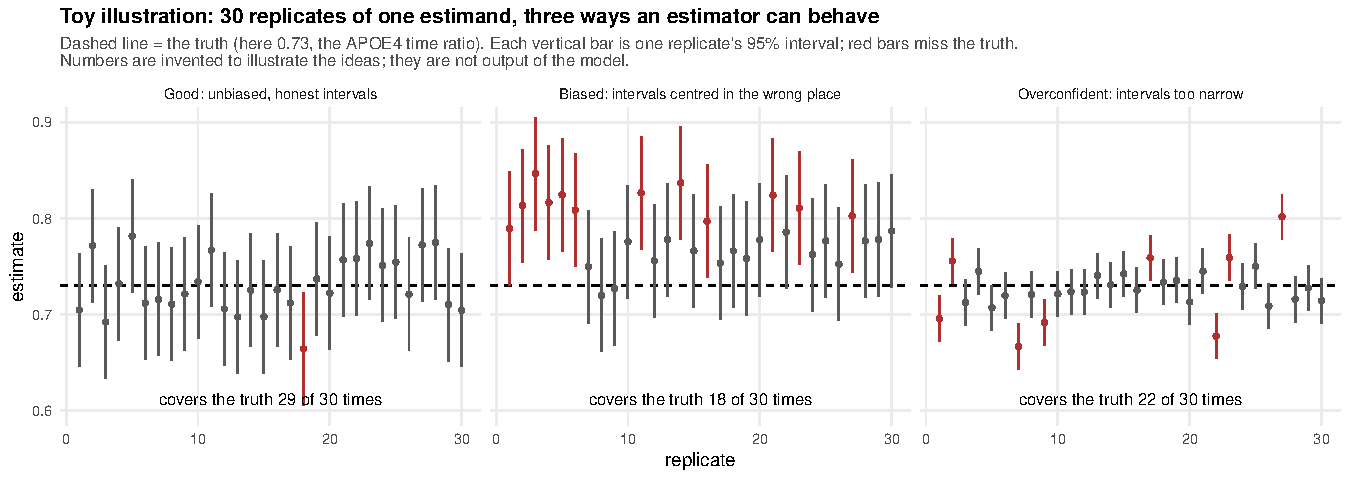
\includegraphics[width=\textwidth]{fig_doc2_bias_coverage.pdf}
\caption{A toy illustration of what the study is looking for. Left: what success looks like; the intervals catch the truth almost every time, missing occasionally, as 95\% intervals should. Middle: a biased estimator, which is centred too high, so many intervals miss. Right: an overconfident estimator, centred correctly but with intervals too narrow. These numbers are invented; they are not results from the model.}
\end{figure}

\subsection{Monte Carlo error: the simulation is itself uncertain}

With a finite number of replicates, every measure above is itself an estimate with its own uncertainty. The study reports a \emph{Monte Carlo standard error} alongside bias and coverage so you can tell real problems from bad luck.

\[
\text{MCSE}(\text{bias}) = \frac{\operatorname{SD}_r(\hat\theta_r - \theta_r)}{\sqrt R},
\qquad
\text{MCSE}(\text{coverage}) = \sqrt{\frac{c\,(1-c)}{R}}.
\]

For coverage the practical consequence is this. If the model's true coverage really is 95\%, the coverage you observe will usually fall within these ranges just by chance:

\begin{center}
\begin{tabular}{@{}c c c@{}}
\toprule
Replicates & One MCSE & Usual range if the truth is 95\% \\
\midrule
40 & 3.4 points & about 88\% to 100\% \\
100 & 2.2 points & about 91\% to 99\% \\
\bottomrule
\end{tabular}
\end{center}

\begin{caution}[Do not over-read small differences]
With 40 replicates, an observed coverage of 90\% is not evidence of a problem. An observed coverage of 75\% is. The \code{rate\_only}, \code{low\_cure} and \code{null} scenarios have 40 replicates each in the \code{small} tier, so judge them with this in mind.
\end{caution}

\subsection{Person-level measures}

\begin{itemize}
  \item \textbf{P(accumulator) by true state.} The average probability the model assigns to being an accumulator, among the true C, true L and true P people. A good model gives C people low values and P people high values. L people are genuinely ambiguous, because their scans are flat, so they should land in between.
  \item \textbf{AUC.} The chance that a randomly chosen true accumulator gets a higher probability than a randomly chosen true non-accumulator. A value of 0.5 is a coin toss and 1.0 is perfect sorting.
  \item \textbf{Accuracy.} The share of people classified correctly when we call anyone above 0.5 an accumulator.
  \item \textbf{Starting-age error and coverage}, separately for true P and true L people. Expect the L group to be much worse: their scans say only ``has not started by the last visit'', not when they will.
\end{itemize}

\subsection{A known trap: correlating estimates}\label{sec:pitfall}

The main README warns about a specific mistake. If you take each person's estimated starting age and estimated speed and correlate them across people, you find a clear negative correlation. It is tempting to read this as ``people who start late go fast''. But the README showed that the same correlation appears on data simulated with starting age and speed \emph{independent by construction}. It comes from how the model estimates them, not from biology. The reason is that a set of scans fits ``started late and went fast'' about as well as ``started early and went slow'', so the two estimates move together.

The simulation measures this directly. In every replicate the truth has starting age and speed independent. The study computes the correlation two ways:

\begin{itemize}
  \item \textbf{from the per-person summary estimates}, which is the trap and should show a spurious negative value;
  \item \textbf{within each posterior draw}, then averaged, which is the correct method and should be close to zero.
\end{itemize}

If the second is near zero while the first is not, the simulation confirms the README's warning on fresh data.

\subsection{The output}

\code{summarise\_sim("small")} writes to \code{figures/sim/small/}:

\begin{center}
\small
\begin{tabularx}{\textwidth}{@{}l X@{}}
\toprule
File & Contents \\
\midrule
\code{performance.csv} & One row per scenario and quantity: truth, mean estimate, bias with MCSE, relative bias, empirical SE, RMSE, coverage with MCSE, mean width. \\
\code{subject\_level.csv} & Per-scenario averages of the person-level measures, R-hat and run time. \\
\code{subject\_level\_per\_rep.csv} & The same, one row per replicate. \\
\code{fig\_sim1\_intervals.pdf} & Every replicate's estimate and 95\% interval against the truth. Intervals that miss are red. \\
\code{fig\_sim2\_coverage\_bias.pdf} & Coverage and bias for every headline quantity, with Monte Carlo error bars. \\
\code{fig\_sim3\_rate\_curve.pdf} & The true rate curve, the spread of estimated curves, and coverage at each level. \\
\code{fig\_sim4\_subjects.pdf} & P(accumulator) by true state, AUC, the correlation trap, and starting-age coverage. \\
\bottomrule
\end{tabularx}
\end{center}

It also prints a compact table for each scenario to the console.

%=====================================================================
\section{Making it run on a laptop}

\subsection{The problem}

Measured on an 11-core M3 Pro MacBook, one fit of the full 1,101-person cohort costs:

\begin{center}
\begin{tabular}{@{}l r@{}}
\toprule
Step & Time \\
\midrule
Compile the model & about 70 s \\
One MCMC iteration, full cohort & 0.117 s \\
One MCMC iteration, per person & about 0.0001 s \\
The reported analysis, 3 chains of 10,000 iterations & about 1 hour \\
\bottomrule
\end{tabular}
\end{center}

A naive simulation that compiled and ran the full analysis for each of 100 replicates would take about 100 hours. That is four days of a laptop doing nothing else.

\subsection{Three things that bring it down}

\begin{enumerate}
  \item \textbf{Compile once per worker} (Section~\ref{sec:fit}). Compile cost drops from once per replicate to once per worker.
  \item \textbf{Run eight replicates at once.} Replicates do not depend on each other, so \code{sim\_run.R} starts a pool of worker processes, by default eight. Each worker compiles its own model and then takes the next unfinished replicate from a shared queue. A worker that finishes early immediately picks up more work.

  The M3 Pro has five fast cores and six slower efficiency cores. With eight workers busy, each runs about 1.3 times slower than a lone process, so eight workers deliver roughly six times the throughput of one. Eight compiled 400-person models used about 3.6\,GB of memory in total, well within the machine's 18\,GB.
  \item \textbf{Tiers sized to the machine.} Cost per iteration grows in proportion to the number of people, so a 400-person cohort is almost three times cheaper per iteration than the full one. The study is split into tiers:
\end{enumerate}

\begin{center}
\small
\begin{tabularx}{\textwidth}{@{}l c c X c@{}}
\toprule
Tier & People & Chains $\times$ iterations & Replicates & Time with 8 workers \\
\midrule
\code{pilot} & 250 & $2\times400$ & 2, 1, 1, 1 across the four scenarios & about 2 min \\
\code{bench} & 400 & $2\times200$ & one per worker & about 1.5 min \\
\code{small} & 400 & $3\times3{,}000$ & 100 \code{fitted}; 40 each of the other three & about 4 hours \\
\code{full} & 1,101 & $3\times6{,}000$ & 40 \code{fitted} & about 4 hours \\
\bottomrule
\end{tabularx}
\end{center}

Run on a single process, \code{small} and \code{full} would each take about a day. The \code{pilot} tier only checks that everything connects end to end; its numbers mean nothing, because 400 iterations is far too short. The \code{bench} tier measures how fast your machine actually runs with every worker busy, and saves that rate so later time estimates are calibrated to your machine.

\begin{caution}[The 400-person tier is a different study size]
Results from \code{small} describe how the model behaves with 400 people. Intervals will be wider than with 1,101, and some problems that appear at 400 may shrink at 1,101. The \code{full} tier is the one that speaks directly to the real study.
\end{caution}

\subsection{Checkpointing: you can always stop}

Each replicate is written to its own file in \code{results/sim/<tier>/} the moment it is scored. Running the same tier again skips every replicate that already has a file. If you need your laptop back, stop the run; when you restart it, you lose at most the replicates that were in progress, one per worker.

A replicate that fails is not lost silently. Its error message is written to an \code{err\_*.rds} file, listed at the end of the run, and retried automatically the next time the tier is run.

\Needspace{14\baselineskip}
\subsection{Running it}

From the project root:

\begin{verbatim}
source("run_simulation.R")
run_simulation("pilot")                 # 2 min: does it connect?
run_simulation("bench")                 # 2 min: calibrate the time estimates
run_simulation("small", dry_run = TRUE) # print the plan and time estimate only
run_simulation("small")                 # about 4 h
run_simulation("full")                  # about 4 h
summarise_sim("small")                  # re-draw tables and figures at any time
sim_progress("small")                   # from another R session, while it runs
\end{verbatim}

Every setting can be overridden. The first line below adds the \code{rate\_only} test at the real study size. The second matches the reported analysis's chain length exactly; 24 replicates of 10,000 iterations cost the same as 40 of 6,000.

\begin{verbatim}
run_simulation("full", scenarios = "rate_only", n_rep = 20)  # about 2 h
run_simulation("full", n_iter = 10000, n_rep = 24)           # about 4 h
\end{verbatim}

For a long run from a terminal, keep the Mac awake with:

\begin{verbatim}
caffeinate -i Rscript -e 'source("run_simulation.R"); run_simulation("small")'
\end{verbatim}

Progress for a running tier is written to \code{results/sim/<tier>/log.txt}.

%=====================================================================
\section{How to read the results}

This section says what success and failure look like in each scenario.

\begin{center}
\small
\begin{tabularx}{\textwidth}{@{}l X X@{}}
\toprule
Scenario & Reassuring & Worrying \\
\midrule
\code{fitted} & Coverage near 95\% for the ORs, TRs and RRs, with bias small next to the empirical SE. Crossing ages and cure fractions close to the truth. & Coverage well below 95\% for a headline effect, or a consistent bias in one direction. \\
\code{rate\_only} & \code{TR\_apoe4} intervals mostly contain 1, and \code{RR\_apoe4} estimates centre near 1.5. & \code{TR\_apoe4} reported well below 1 while \code{RR\_apoe4} is pulled toward 1. That means faster is being read as earlier, which would undermine the real-data headline. \\
\code{low\_cure} & \code{pi\_bar} near 0.95 and cure fractions near 5\%. & Cure fractions well above 5\%: the model is inventing never-accumulators. \\
\code{null} & About 95\% of intervals for each OR, TR and RR contain 1, so false alarms happen about 5\% of the time. & Effects declared far more often than 5\%: the model manufactures findings. \\
\bottomrule
\end{tabularx}
\end{center}

\paragraph{Always check R-hat before blaming the model.} Some replicates will not have fully converged, because the tiers use shorter chains than the reported analysis: 3,000 or 6,000 iterations against 10,000. The main README reports a worst R-hat of 1.56 at 5,000 draws, falling to 1.07 at 10,000. If intervals that miss the truth cluster in replicates with high R-hat, the problem is run length, not the model. Rerun with longer chains and fewer replicates, at the same total cost, to tell the two apart.

\paragraph{Expect some quantities to be harder than others.} The person-level starting age for L people is fundamentally hard: their data contain no rise. The top of the rate curve rests on few scans and leans on the prior. The spreads $\sigma_\alpha$ and $\sigma_\delta$ are usually harder to pin down than the covariate effects. Poorer performance there is expected and does not by itself indicate a fault.

%=====================================================================
\section{What this study can and cannot tell you}

\begin{enumerate}
  \item \textbf{It is a best case.} The fake data come from the model's own equations, so the model is exactly right about how the data were made. Real data will not be so cooperative. Passing this test is necessary for trusting the model, but not sufficient. Failing it is serious, because a model that cannot recover its own world will not recover the real one.
  \item \textbf{It tests one point.} Each scenario sets the truth at one particular set of values. Behaviour could differ elsewhere, for example with a much slower rate curve or much shorter follow-up.
  \item \textbf{The design is held fixed on purpose.} Results apply to the ADNI visit pattern. That is the point: it is the design the real analysis used.
  \item \textbf{Chains are shorter than the reported analysis.} See the R-hat note above.
  \item \textbf{The crossing-age comparison is slightly uneven.} The true crossing age averages over the people who really are accumulators. The estimated one averages over the people the model classifies as accumulators, those with probability above 0.5 within each draw. Misclassification can shift the estimate a little even if everything else is right.
  \item \textbf{The cure-fraction truth is a population value.} It comes straight from the scenario's parameters. The share of non-accumulators in any one fake cohort varies around it by chance.
  \item \textbf{Measurement-noise knots are fixed to the real cohort.} The noise curve's spline knots are always taken from the real scans, never re-placed for each fake cohort or subsample. Otherwise ``the true noise curve'' would mean a slightly different function in every replicate.
\end{enumerate}

%=====================================================================
\section{File and function reference}

\begin{center}
\small
\begin{tabularx}{\textwidth}{@{}l >{\raggedright\arraybackslash}p{5.3cm} X@{}}
\toprule
File & Key functions & Job \\
\midrule
\code{run\_simulation.R} & & Entry point. Loads the model and every file below. \\
\code{sim\_truth.R} & \code{sim\_truth}, \code{sim\_estimands} & The four scenarios, and their truth values on the reported scales. \\
\code{sim\_generate.R} & \code{simulate\_cohort}, \code{sim\_design}, \code{sim\_var\_basis} & Draw one fake cohort on the real design. Choose the design for a tier. Fix the noise basis. \\
\code{sim\_fit.R} & \code{sim\_compile}, \code{feasible\_inits}, \code{sim\_fit} & Compile once. Make starting values possible. Fit one replicate on the compiled model. \\
\code{sim\_summarise.R} & \code{score\_replicate}, \code{performance\_table}, \code{subject\_table}, \code{summarise\_sim} & Score one fit against its truth. Aggregate a tier into tables and figures. \\
\code{sim\_run.R} & \code{run\_simulation}, \code{sim\_tiers}, \code{sim\_plan}, \code{sim\_job}, \code{sim\_progress} & Tiers, the worker pool, checkpointing, time estimates, progress. \\
\bottomrule
\end{tabularx}
\end{center}

\paragraph{Random seeds.} Every replicate's random numbers are fixed by its replicate number and by its scenario's position in the tier's list of scenarios, so any replicate can be regenerated exactly. The fake cohort uses one seed and the MCMC uses a second, offset seed, so changing the sampler settings never changes the fake data. Because the seed follows the position and not the name, running a single scenario on its own, for example \code{scenarios = "rate\_only"}, reuses the random numbers of the first scenario in a default run. The truth differs, so the cohorts differ, but they share the same underlying random draws.

%=====================================================================
\section*{Glossary}
\addcontentsline{toc}{section}{Glossary}

\begin{description}[leftmargin=0pt,itemsep=3pt]
  \item[Estimand] A quantity we want to know, such as the APOE4 odds ratio.
  \item[Replicate] One complete cycle of making fake data, fitting, and scoring.
  \item[Scenario] One choice of the true parameter values.
  \item[Posterior draws] The collection of plausible parameter values a Bayesian fit produces. Their spread expresses uncertainty.
  \item[Posterior median] The middle of the posterior draws; used here as the single best estimate.
  \item[95\% credible interval] The range containing the middle 95\% of the posterior draws.
  \item[MCMC] Markov chain Monte Carlo, the random-walk method that produces posterior draws.
  \item[Chain] One run of MCMC. Several chains from different starts are compared to check they agree.
  \item[Burn-in] The early part of each chain, discarded because the walker has not yet found the plausible region.
  \item[R-hat] A check of whether chains agree. Near 1 is good; much above 1 means run longer.
  \item[Bias] Average difference between estimate and truth across replicates.
  \item[Coverage] Share of replicates whose interval contains the truth. Should be near 95\% for 95\% intervals.
  \item[Monte Carlo standard error] The uncertainty in a simulation result caused by using a finite number of replicates.
  \item[Odds ratio, time ratio, rate ratio] Multiplicative effects of a covariate on the odds of ever accumulating, on the time until starting, and on speed once started. A value of 1 means no effect.
  \item[SUVR, Centiloid] Two scales for amyloid PET. Centiloid is a linear rescaling of SUVR; 24 Centiloid is the positivity threshold.
  \item[Compile] Translate the model into fast machine code before running it. Slow once, fast afterwards.
\end{description}

\end{document}
